\documentclass[a4paper,12pt]{article}
\usepackage{fancyhdr}
\usepackage{lastpage}
\usepackage{geometry}
\usepackage{listings}
\usepackage{datetime}
\usepackage{xeCJK}
\usepackage{hyperref}
\usepackage{amsmath}
\usepackage{graphicx}
\usepackage{float} % 加入 float 宏包以使用 [H]
\usepackage{longtable}

\geometry{left=2.5cm, right=2.5cm, top=2.5cm, bottom=2.5cm}
\pagestyle{fancy}
\setCJKmainfont{Noto Sans TC}
% 英文字體 consolas
\setmonofont{Consolas}
% 設定內文文字大小
\renewcommand{\normalsize}{\fontsize{12pt}{\baselineskip}\selectfont}

% 設定頁首
\fancyhf{}
\fancyhead[L]{Volume Rendering and Gradient Visualization(HW3)}
\fancyhead[R]{\today}
\fancyfoot[C]{\thepage/\pageref{LastPage}}

\title{Volume Rendering and Gradient Visualization(HW3)}
\author{01057033洪銘均}
\date{\today}

\begin{document}
\maketitle
\tableofcontents
\newpage

\section{程式概述}
該程式在作業2的基礎下,加入Volume Rendering,利用Raycasting對Volume做採樣,加總後做視覺化。


\section{運行結果}

\begin{figure}[h]
    \centering
    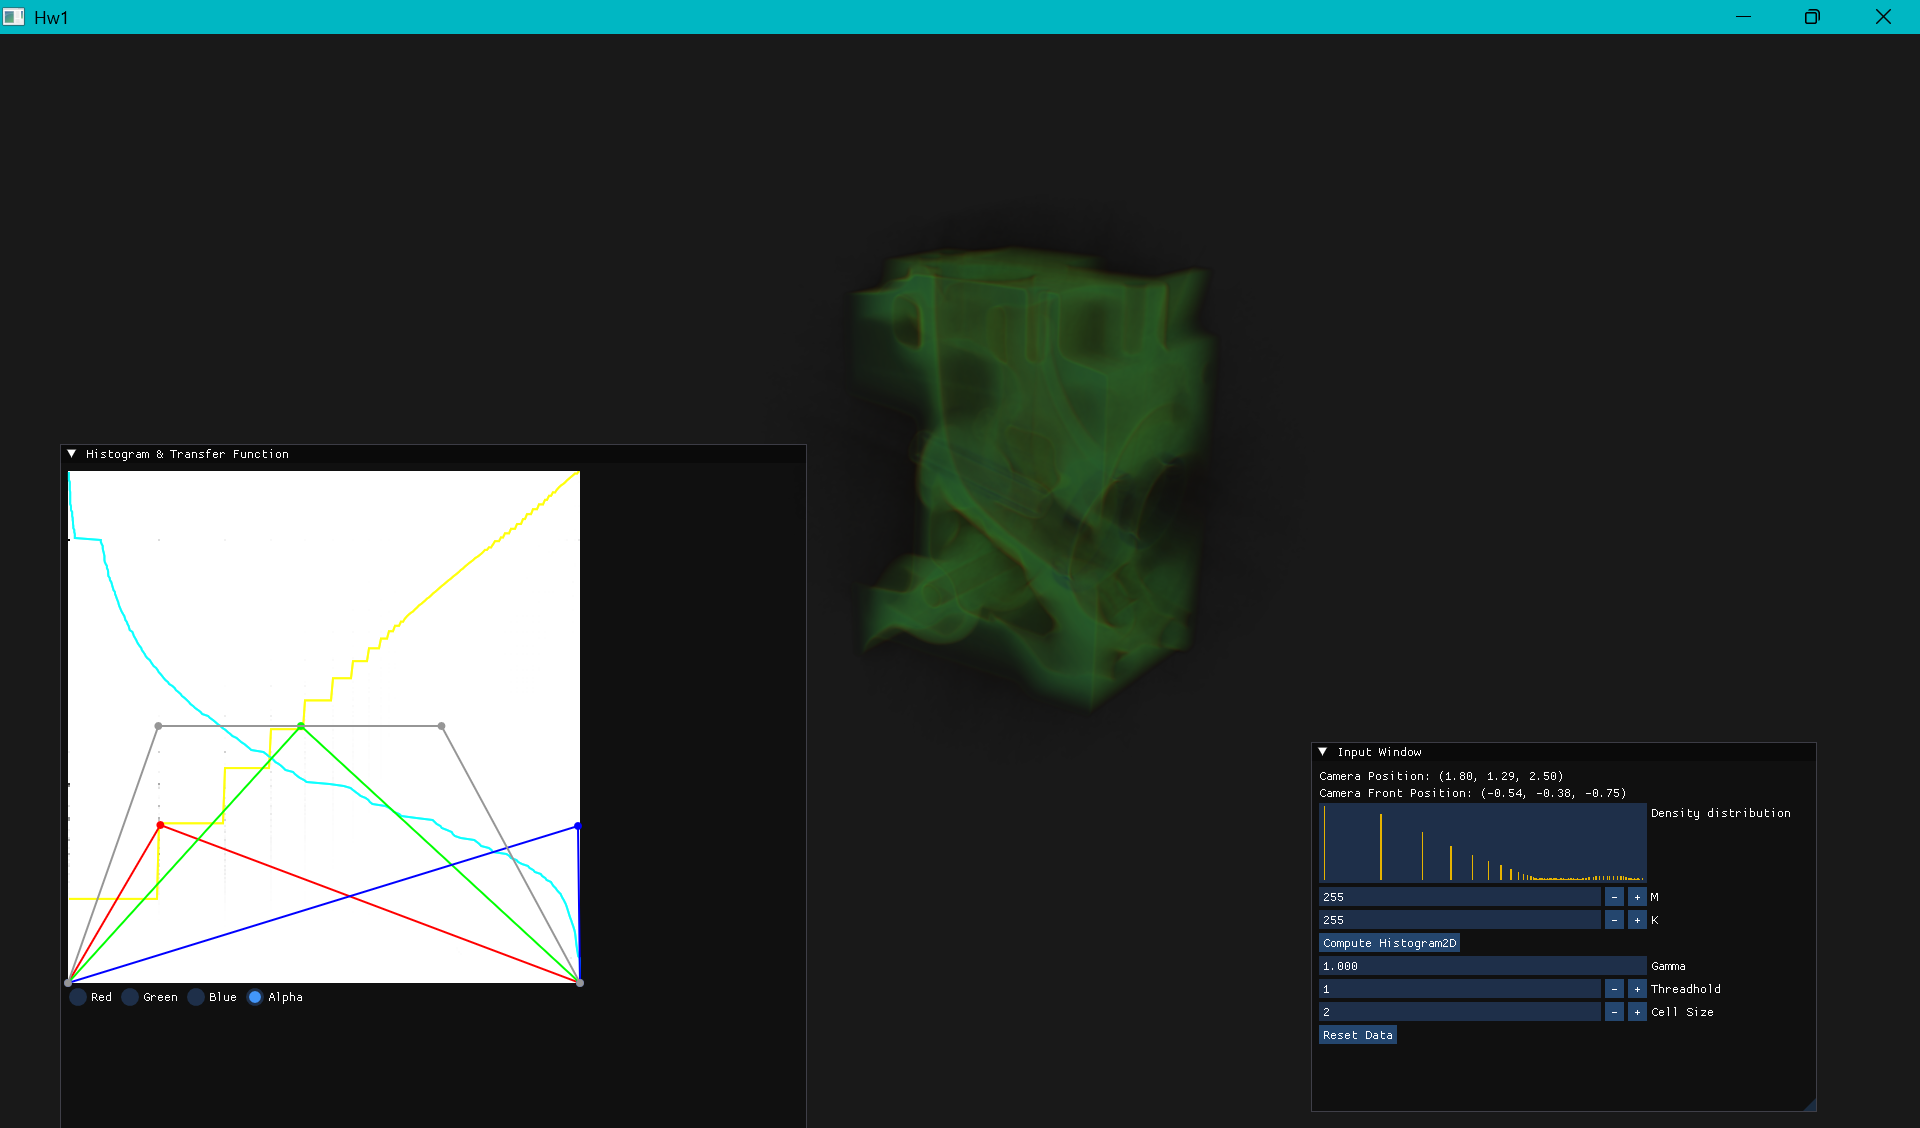
\includegraphics[width=0.8\textwidth]{img/img0.png}
\end{figure} \\
圖中為引擎的Volume Rendering視覺化,其中紅色為硬度值較低的體積,藍色為較硬的。\\

\begin{figure}[h]
    \centering
    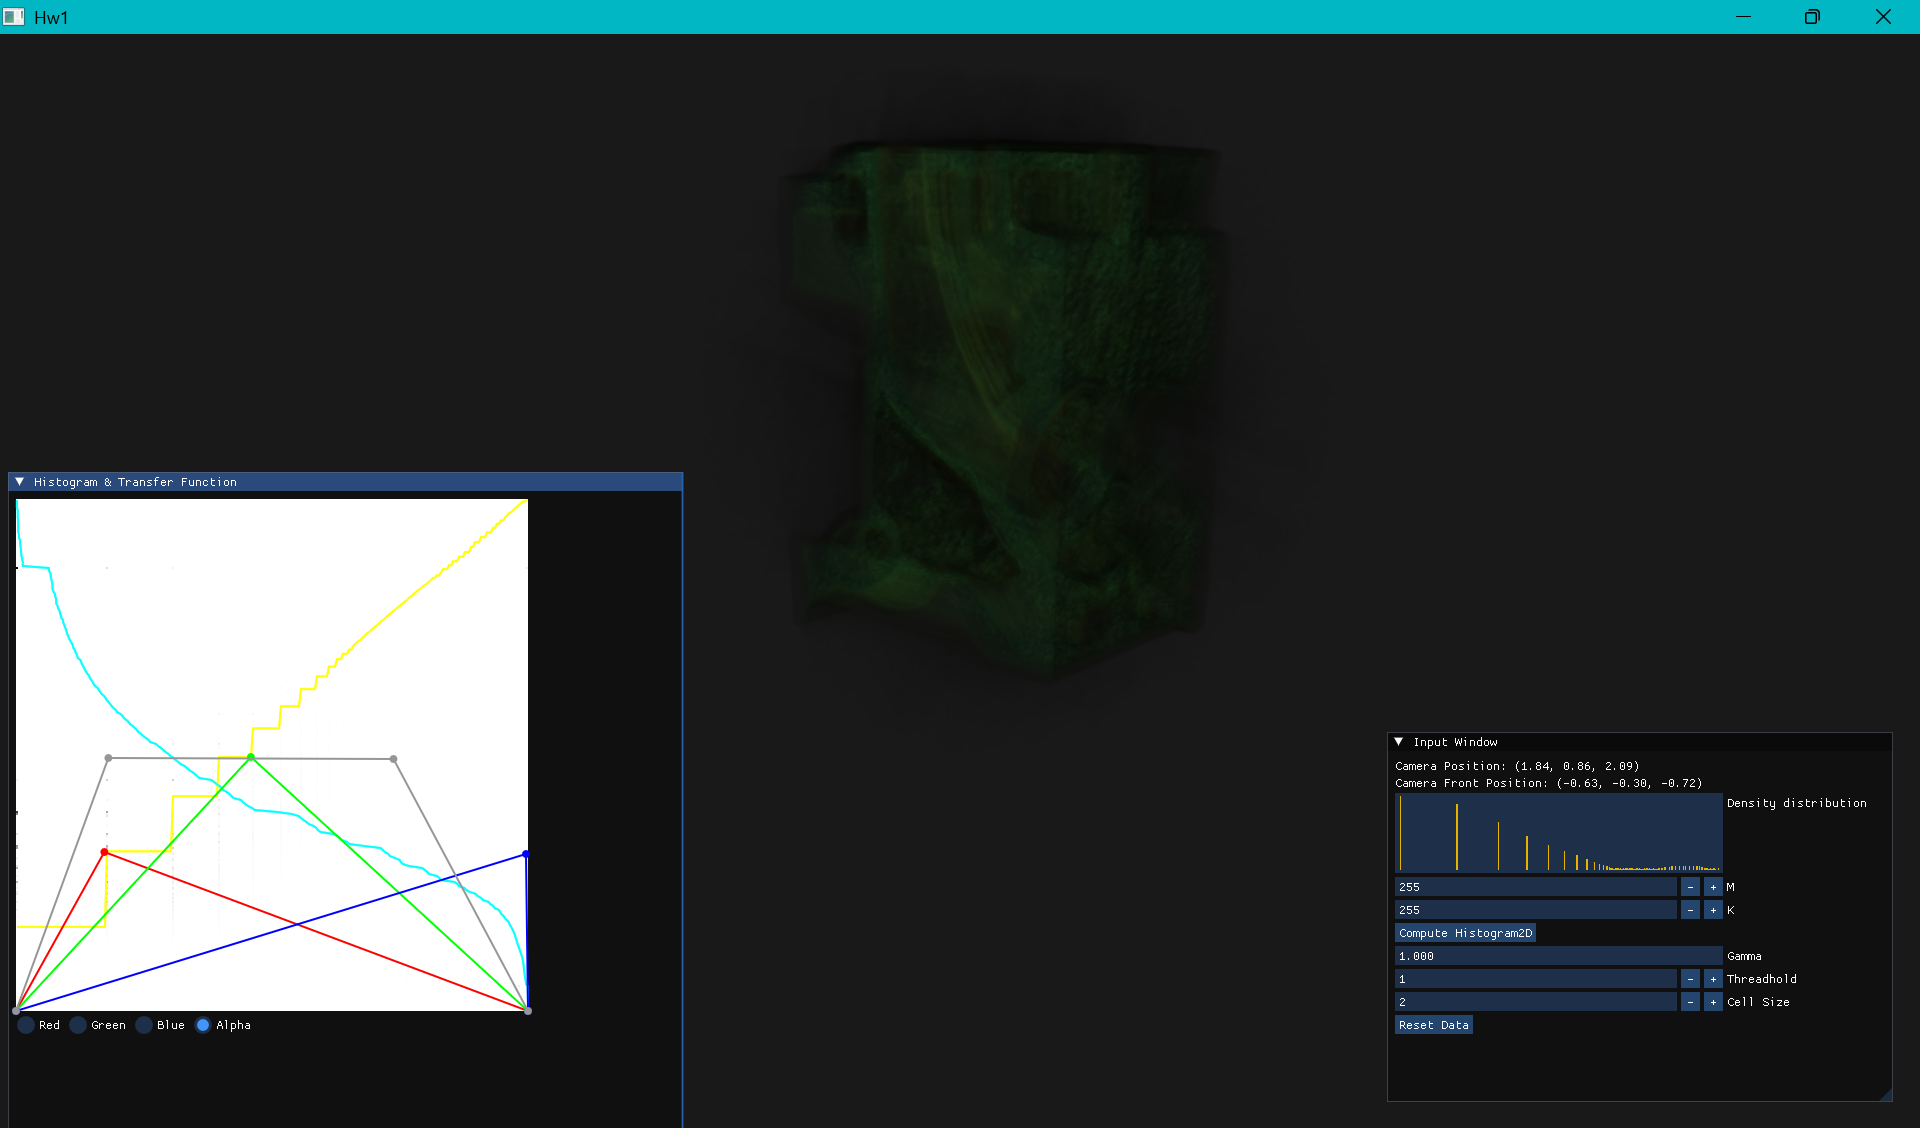
\includegraphics[width=0.8\textwidth]{img/img1.png}
\end{figure} \\
圖中為引擎的Volume Rendering視覺化,並且加入了Phong Shading,硬度的顏色分配與上圖相同,在有Phong Shading的圖片可以看到,邊緣位置有Shading所呈現的凹凸紋理。\\

\section{心得}
這次作業成功使用Raycasting完成Volume Rendering,並且加入Phong Shading使其能夠更詳細的標線出表面的凹凸紋理,在時限Volume Rendering時還有再多修改Transfer Function的折線圖部分,原本折線圖是與Gradient-Distrubtion圖分開,獨立三張圖,後來將Gradient-Distrubtion圖與折線圖合併方便調整Transfer Function。

\end{document}

% xelatex  --max-print-line=10000 -synctex=1 -interaction=nonstopmode -file-line-error -recorder .\codebook.tex 
